\item[\ding{226}]\textbf{Strategie Combiné de l'Oscillateur Stochatique et de la 
Moyenne Mobile Convergence Divergence (avec les nouveaux paramètres).}

\begin{center}     \textbf{"BRVM-Agriculture"}  \end{center}
\begin{figure}[h]
    \centering
    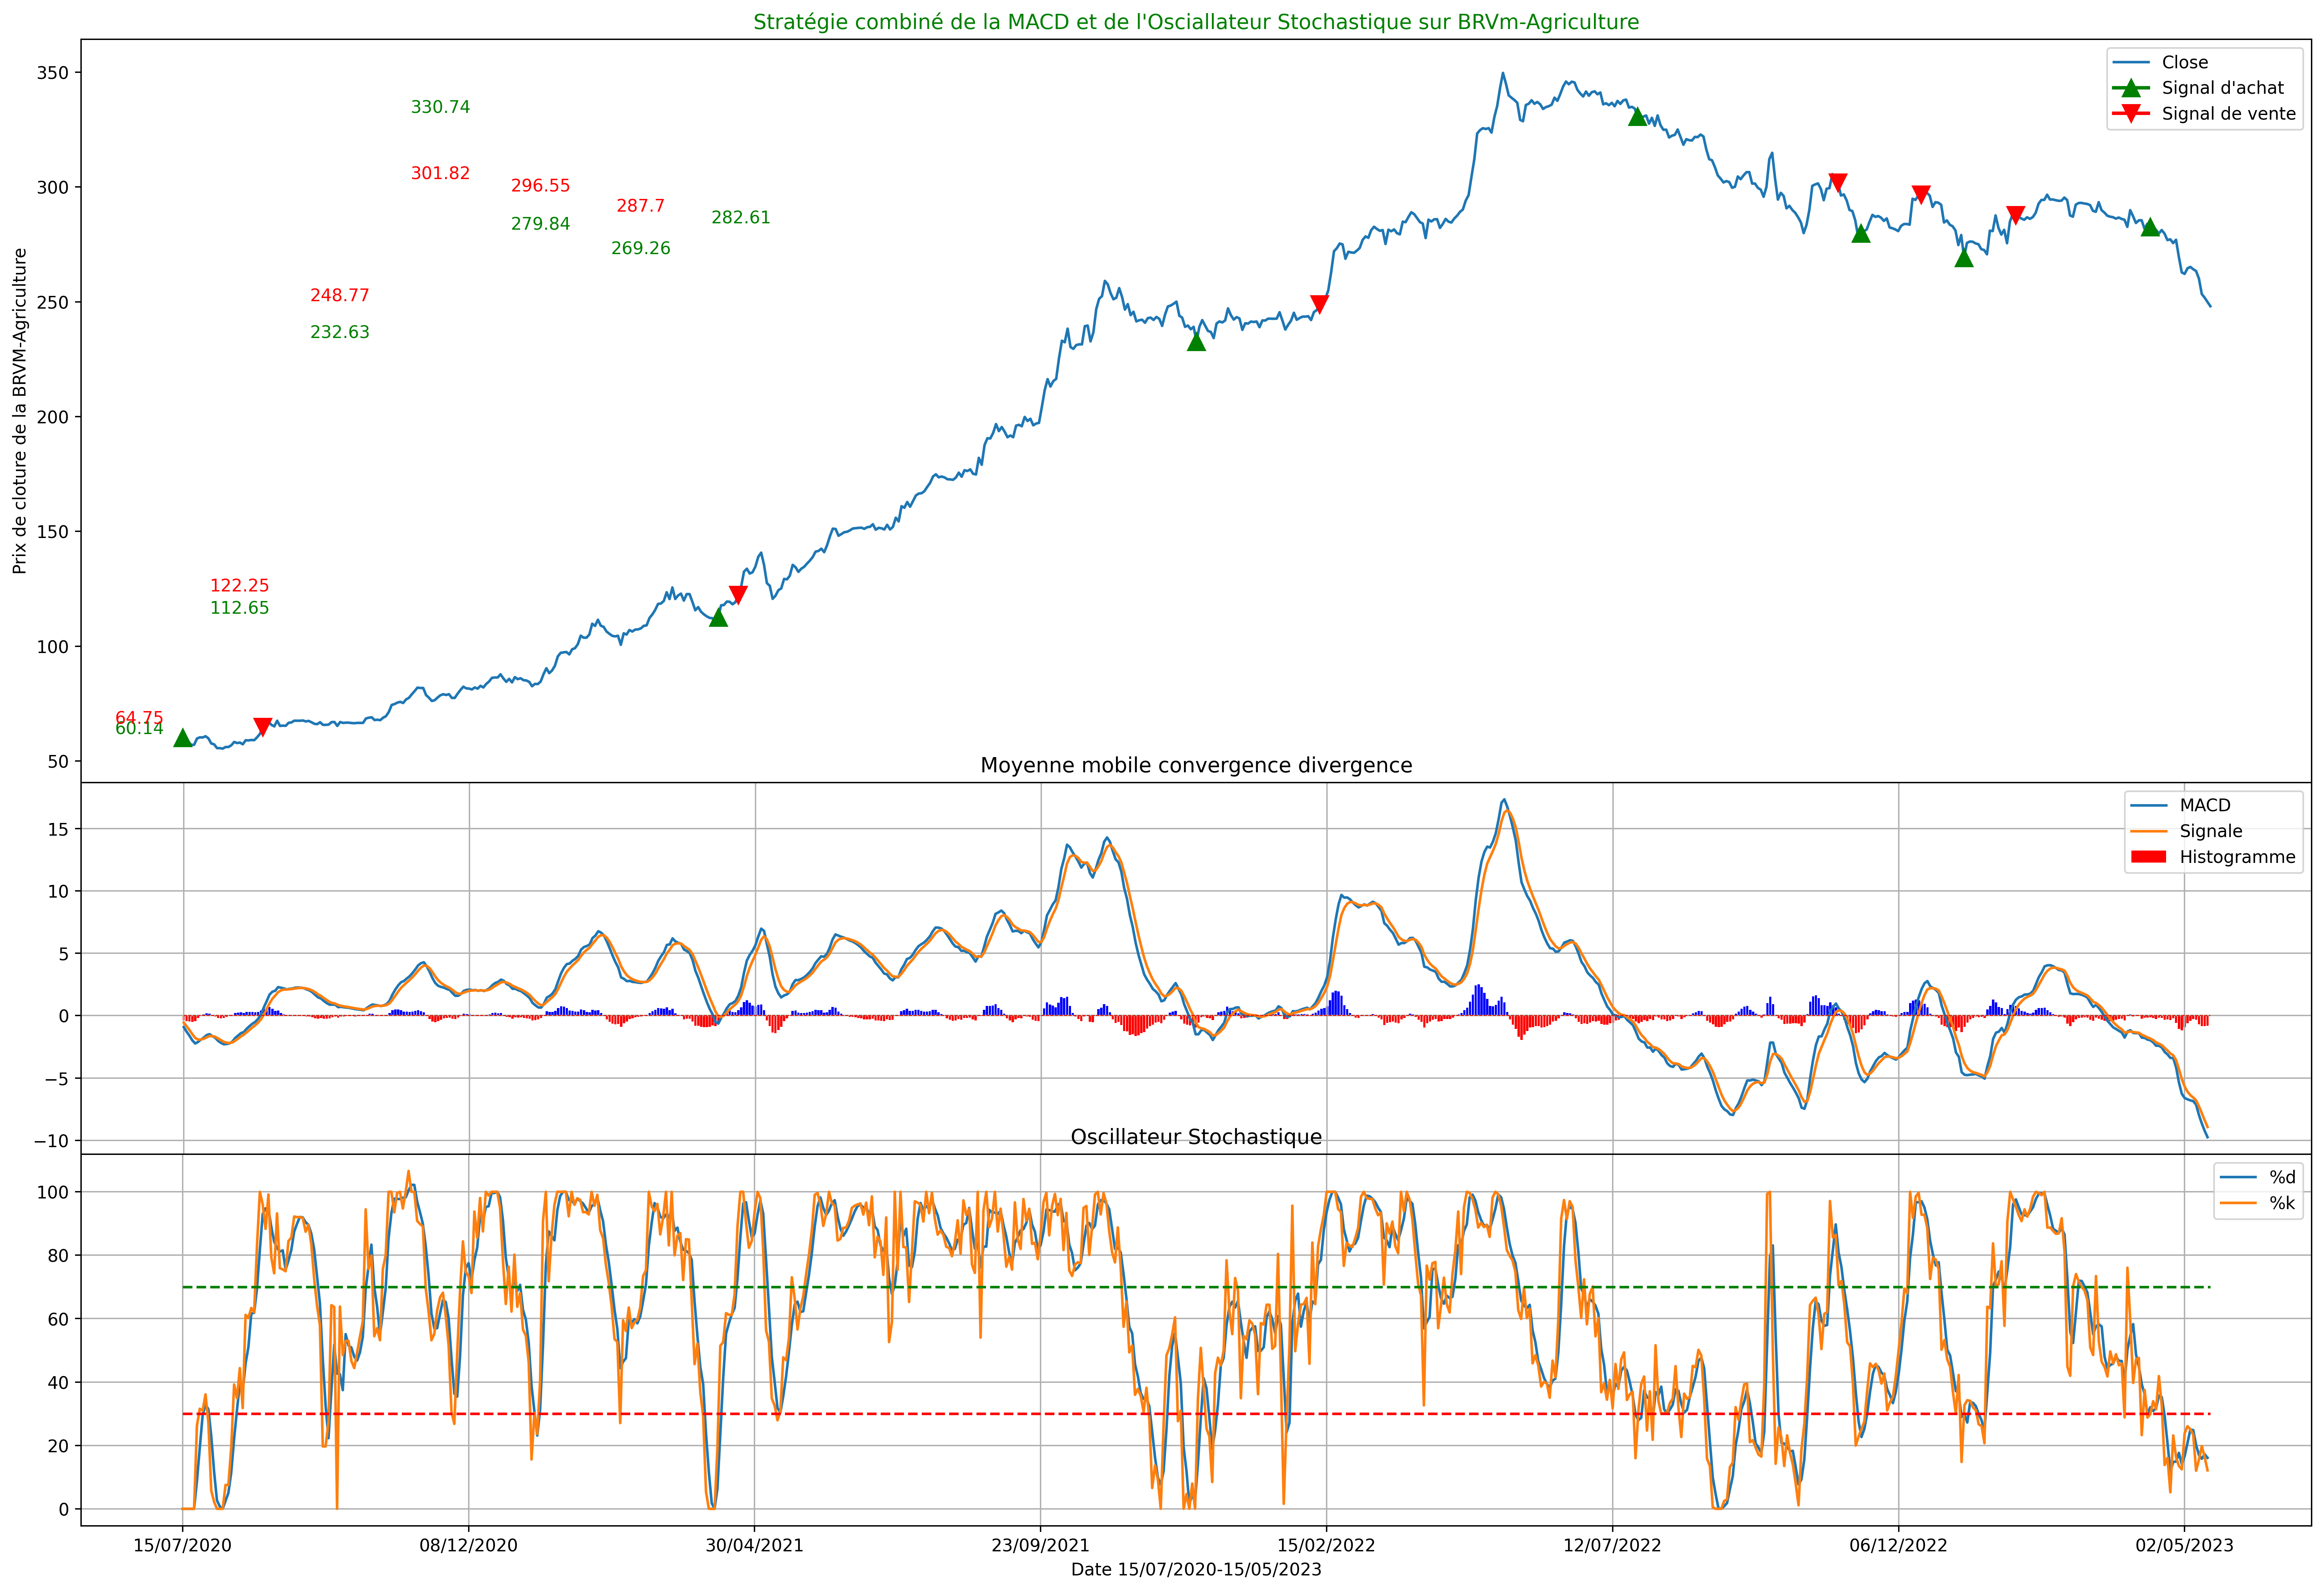
\includegraphics[width=1 \textwidth ]{img/MACD-Agri.png}
    \caption{Strategie Combine de MACD et de Stochastique sur l'indice Agriculture}
    \label{fig:Strategie Combine de MACD et de Stochastique sur l'indice Agriculture}
\end{figure}
\par{La représentation graphique ci-dessus, illustre la courbe du cours de l'indice BRVM-Agriculture , 
la Moyenne Mobile Convergence Divergence , ainsi que l'Oscillateur Stochastique. De cette
représentation graphique, nous pouvons observer que les courbes de l'Oscillateur Stochastique 
dépasse très fréquemment la barre des 70\% ce qui indique à chaque fois que le marché est dans 
un état de surachat ce qui représente un signal de vente. Cependant afin de valider 
ce signal il faut que la MACD soit supérieur à zéro. 
De plus on peut remarquer que 
après le 12 juillet 2022 une fluctuation inhabituelle des cours de l'indice, ce 
qui a générer un faux signal de vente et qui donc a conduit une perte au cours de cette
transaction. Suivant les cours des transactions en haut à gauche (du côté de la courbe des cours
de l'indice) nous pouvons observer que le prix d'achat de la valeur à cette transaction 
était de 330,74 Fcfa et son prix de vente de 301,81 Fcfa. 
Finalement la stratégie combinée
de l'Oscillateur Stochastique et de la Moyenne Mobile Convergence Divergence à donner un 
bénéfice total de \textbf{29,105\%} } 




\begin{center}     \textbf{"BRVM-Services-Publics"}  \end{center}
\begin{figure}[h]
    \centering
    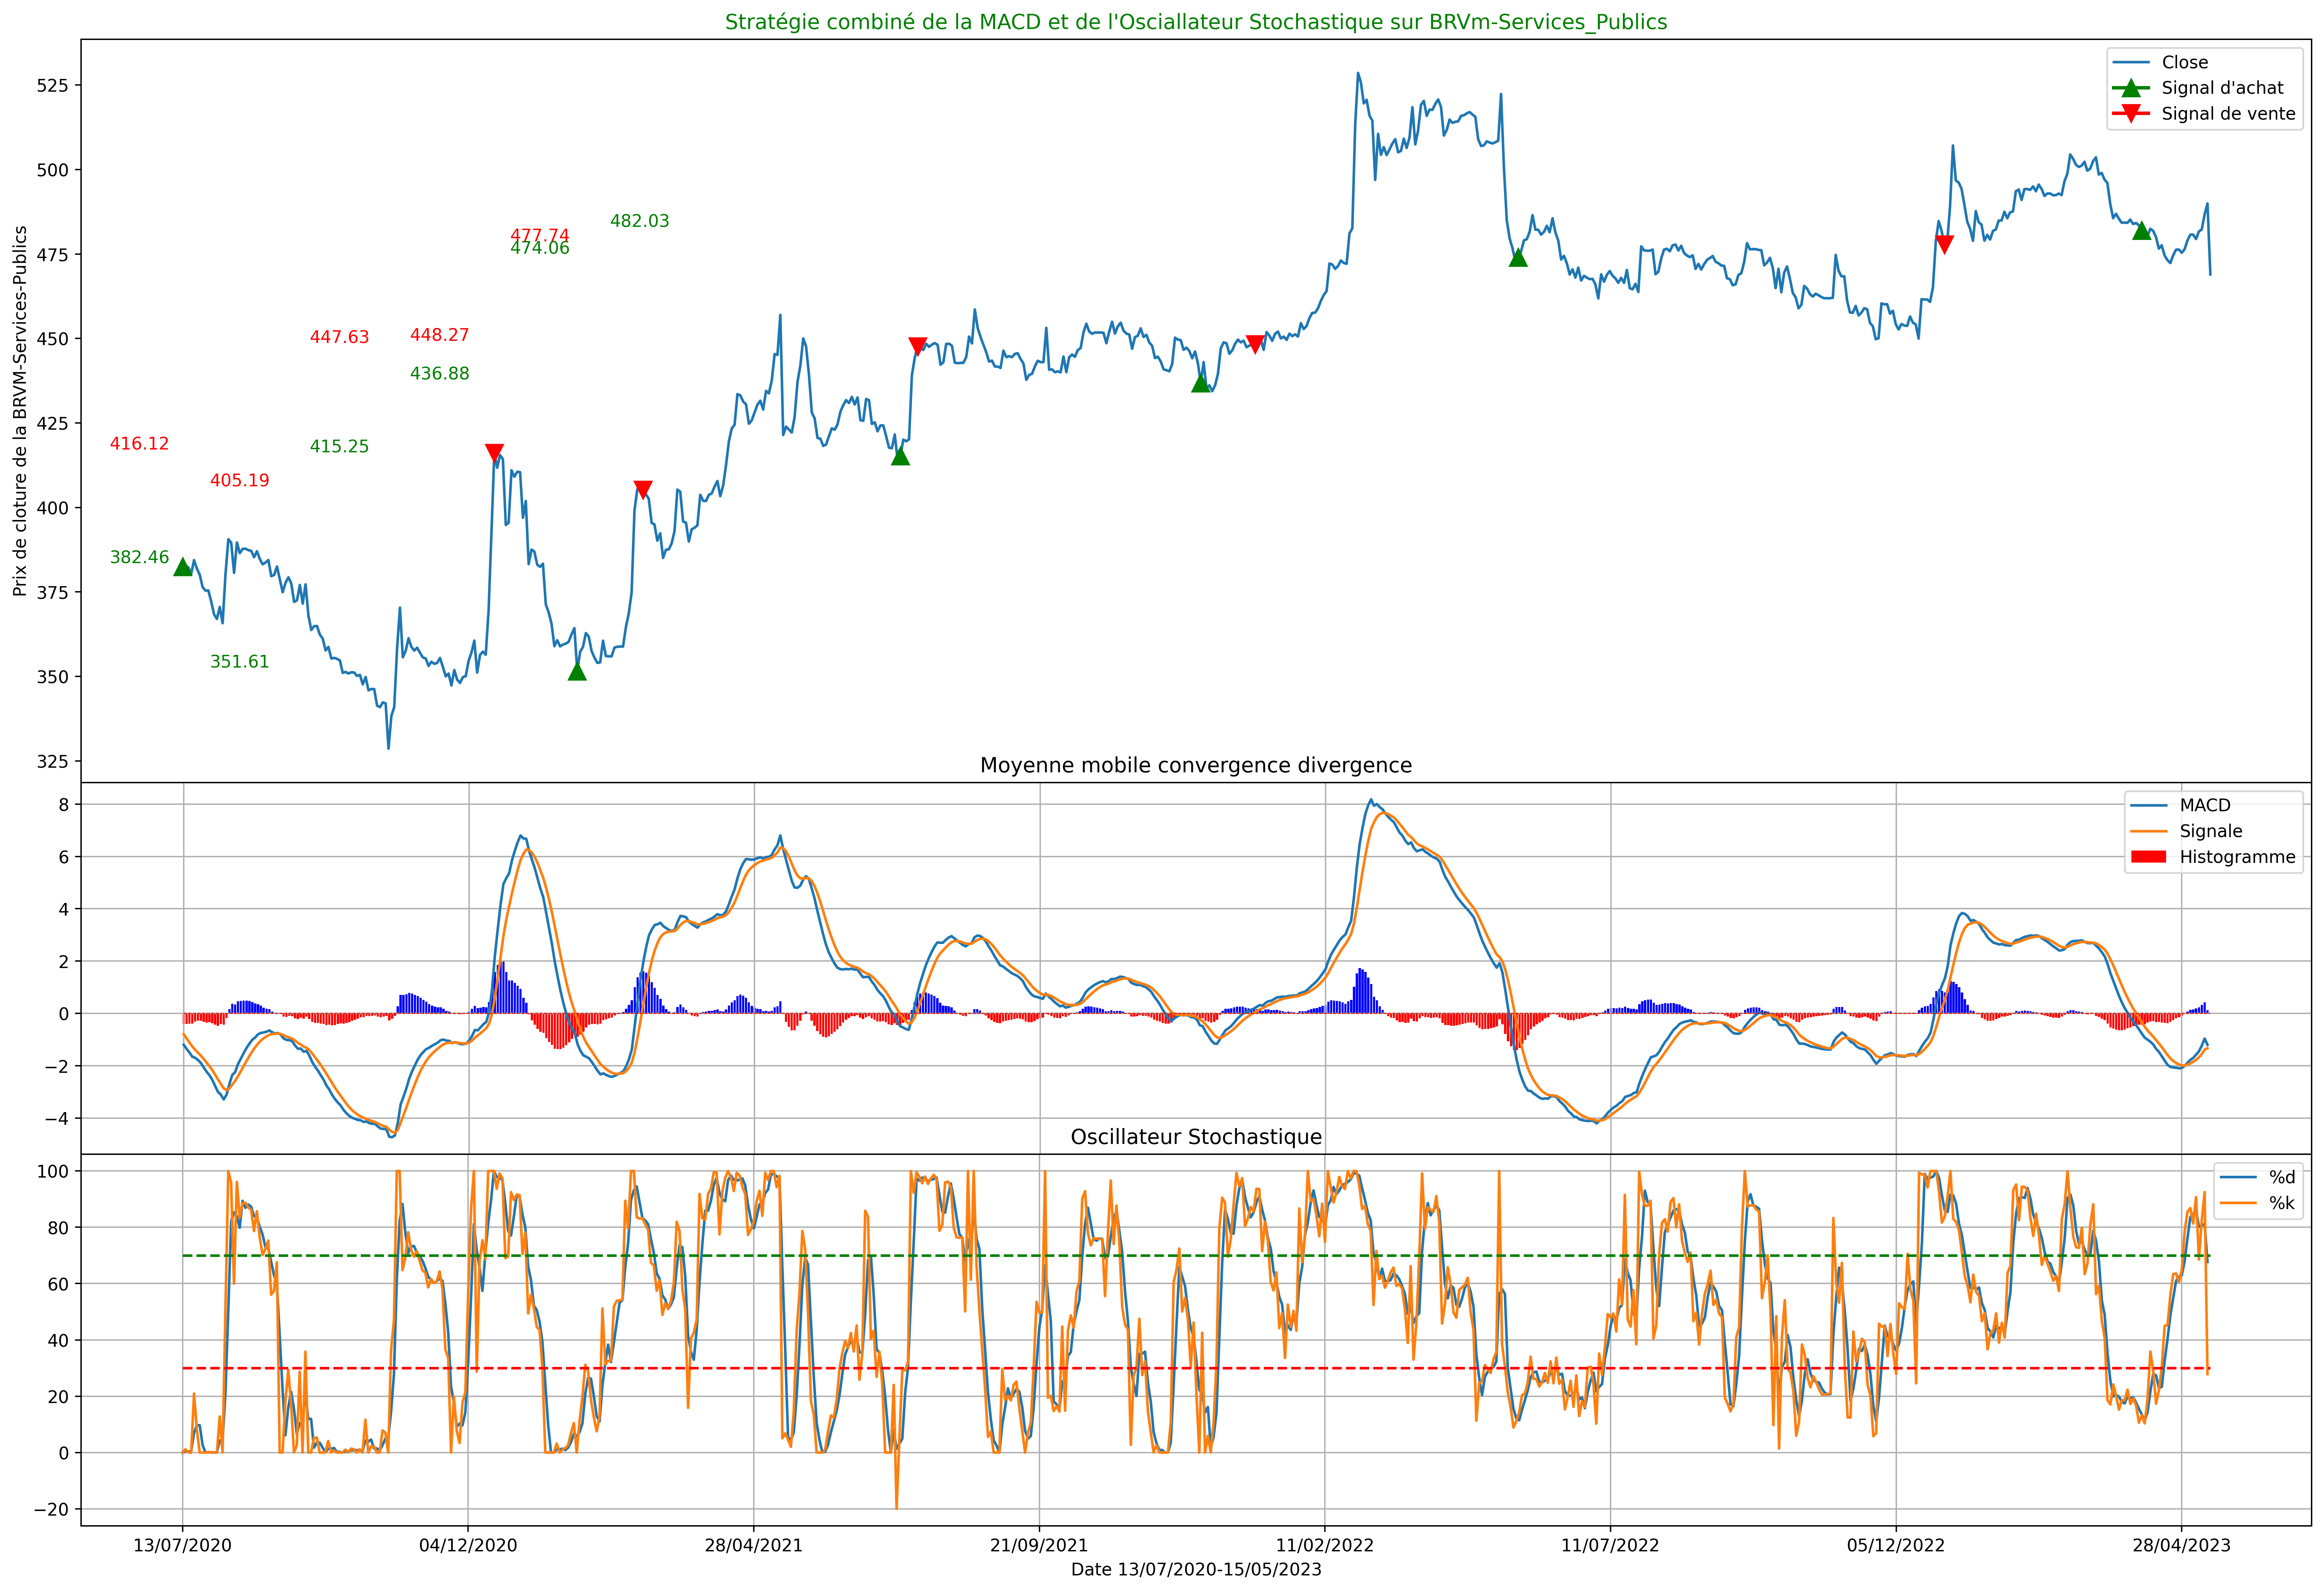
\includegraphics[width=1 \textwidth ]{img/MACD-Public.png}
    \caption{Strategie des Moyennes Mobiles sur la BRVM-Services-Publics}
    \label{fig:Strategie des Moyennes Mobiles sur la BRVM-Services-Publics}
\end{figure}

\par{La figure ci-dessus présente l'application de la stratégie combinée de l'oscillateur 
Stochastique et de la Moyenne Mobile Convergence Divergence sur l'indice BRVM-Service-Publics.
De son analyse il ressort qu'il y a une répartition équitable des signaux d'achat et de vente
générer par la Moyenne Mobile Convergence Divergence. En tout nous avons obtenu 
9 signaux d'achat et de vente dont un signal d'achat final. La transaction
la plus bénéfique réalisé est la deuxième ou le prix d'achat de la valeur était 
de 351,61 Fcfa et son prix de vente de 405,19 Fcfa. Notons que toutes les transactions 
sont positives et que le taux de bénéfice total réalisé à la fin de l'application de 
la stratégie est de \textbf{39,758\&}.

Bien que toute les transaction soit 
positive on observe que le 5eme signal de vente est venu un peut trop tôt 
car dans la suite de l'évolution des cours, le prix de l'indice à dépasser les 
500 Fcfa contre un signal d'achat ou l'indice coutait 474,06 Fcfa. Ce retard est 
d'autant plus remarquable au niveau de la 4eme transaction où le signal de vente est 
venu vraiment très tôt cas juste après le signal de vente l'indice à atteint sont 
cours maximal de \textbf{ 528,59 Fcfa}.}




\subsection{{Interprétation des résultats et vérifications des hypothèses.}}

D'après les analyses, la stratégie des Moyennes Mobile sur l'indice BRVM-Agriculture à 
générer au total de 8 signaux d'achat et de vente et 6 signaux d'achat et de vente 
sur l'indice BRVM-Services-Publics. En ce qui concerne la stratégie
combinée de l'Oscillateur Stochastique et de la Moyenne Mobile Convergence Divergence, 
elle à donner 13 signaux d'achat et de vente pour l'indice BRVM-Agriculture et 
11 signaux d'achat et de vente pour l'indice BRVM-Services-Publics, ce qui fait un total
de 24 signaux. Nous remarquons donc que nombre total de signaux obtenu grâce 
à la stratégie des Moyennes Mobiles ainsi que le nombre total de signaux individuel pour 
chaque indice est inférieur aux signaux obtenu grâce à la stratégie combiné de l'oscillateur
stochastique et de la Moyenne Mobile Convergence Divergence. Alors l'hypothèses selon laquelle 
la méthode des Moyennes Mobiles génère plus de signal d'achat et de ventes que la méthodes
combinée de l'Oscillateur Stochastique et de la des Moyennes Mobiles convergence divergence 
n'est pas vérifier.

De plus il ressort que l'application de la stratégie des moyennes 
mobile à générer un bénéfice total de 367,167\% sur l'indice BRVM-Agriculture et 
un total de 18,01\% sur l'indice BRVM-Services-Publics. Par ailleurs la stratégie 
combinée de l'Oscillateur Stochastique et de la Moyenne Mobile Convergence Divergence
quand à elle a donné un bénéfice total de 29,105\% sur l'indice BRVM-Agriculture 
contre un bénéfice total de 39,758\% pour l'indice BRVM-Service-Publics. 
Il ressort de ces résultats que \textbf{la stratégie des Moyennes Mobile donne plus de 
bénéfice sur l'indice BRVM-Agriculture que sur l'indice BRVM-Services-Publics. 
Alors que la stratégie Combiné de l'Oscillateur Stochastique et de la 
Moyenne Mobile Convergence Divergence donne plus de bénéfices sur 
l'indice BRVM-Service-Public que sur l'indice BRVM-Agriculture}. En somme 
la stratégie des Moyennes Mobiles donne un total de 385,177\% pour les deux indices 
et la méthode combinée de l'Oscillateur Stochastique et de la Moyenne Mobile Convergence Divergence
produit un total de 68,863\% pour les deux indices. Alors l'hypothèses selon laquelle
la  méthode combinée de l'Oscillateur Stochastique et de la Moyenne Mobile Convergence Divergence
génère plus de bénéfices que la méthode des Moyennes Mobile n'est pas vérifié.

\section{Approche de solution}
\par{
Afin d'optimiser au mieux le profil des investisseurs à la Bourse Régional des 
valeurs Mobilière, notamment ceux qui investissent dans le domaine des Services
Publics et de l'Agriculture, entre la stratégie de la 
moyenne mobile et de la méthode Combiné de l'Oscillateur Stochastique et de la 
Moyenne Mobile Convergence Divergence au vu des résultats obtenus dans cet études 
nous recommandons vivement l'utilisation de la stratégie des Moyennes Mobile 
sur l'indice BRVM-Agriculture et l'usage de la méthode Combiné de l'Oscillateur
    stochastique et de la Moyenne Mobile Convergence Divergence sur l'indice 
    BRVM-Services-Publics. De plus dans le cadre de l'application de ces stratégies
    nous recommandons de faire des simulations afin de déterminer les paramètres pour la stratégie des 
    moyennes mobiles qui permettent d'obtenir de meilleur bénéfice pour les tendance 
    futur du marché et l'usage de nos critère de validations des paramètres élaborer dans le 
    cadre de cette étude comparative. 
}




